\begin{frame}[allowframebreaks]{}
    \LARGE Normalizing Flow Models: \\[1.5ex] \textbf{Flow Matching}
\end{frame}

\begin{frame}{From Discrete Flows to Continuous-Time Flows}
\begin{itemize}
    \item So far: a flow is a \textbf{stack of invertible layers}, each designed so its Jacobian determinant is cheap (coupling layers, $1\times1$ convolutions).
    \item \textbf{Continuous normalizing flows (CNFs)} (Chen et al., 2018) replace the stack with a \textbf{vector field}: a network $v_\theta(x, t)$ defines an ODE
    $$
    \frac{dx_t}{dt} = v_\theta(x_t, t),
    $$
    and the flow is the result of integrating it from $t=0$ to $t=1$.
    \item ODE solutions are invertible by construction (integrate backwards), so \textbf{any architecture} can be used: no coupling-layer constraints.
\end{itemize}
\end{frame}

\begin{frame}{CNFs: Likelihood and the Training Bottleneck}
\begin{itemize}
    \item The change of variables formula becomes \textbf{instantaneous}:
    $$
    \frac{\partial \log p(x_t)}{\partial t} = -\,\mathrm{tr}\!\left( \frac{\partial v_\theta}{\partial x_t} \right),
    $$
    a trace instead of a log-determinant.
    \item \textbf{The catch:} training a CNF by maximum likelihood (FFJORD, Grathwohl et al., 2019) requires \textbf{simulating the ODE} and estimating the trace at every training step.
    \item Accurate and architecture-free, but slow and hard to scale to large images. This is the problem flow matching removes.
\end{itemize}
\end{frame}

\begin{frame}{Flow Matching: Simulation-Free Training}
\begin{itemize}
    \item \textbf{Flow Matching (FM)} (Lipman et al., ICLR 2023) trains the same object, a vector field $v_\theta$, \textbf{without ever simulating the ODE}.
    \item Idea: fix a \textbf{target probability path} $p_t$ that moves from noise ($t=0$) to data ($t=1$), with generating field $u_t$, and simply \textbf{regress}:
    $$
    \mathcal{L}_{\mathrm{FM}}(\theta) = \mathbb{E}_{t,\; x \sim p_t} \left\| v_\theta(x, t) - u_t(x) \right\|^2 .
    $$
    \item Problem: $u_t$ for the whole data distribution is unknown in closed form, so this loss cannot be computed directly.
\end{itemize}
\end{frame}

\begin{frame}{Conditional Flow Matching}
\begin{itemize}
    \item Solution: define the path \textbf{per sample pair}: condition on a noise sample $x_0$ and a data sample $x_1$, giving a conditional path $p_t(x \mid x_0, x_1)$ whose field $u_t(x \mid x_0, x_1)$ is known, and regress on that instead:
    $$
    \mathcal{L}_{\mathrm{CFM}}(\theta) = \mathbb{E}_{t,\; x_0,\, x_1,\; x \sim p_t(x \mid x_0, x_1)} \left\| v_\theta(x, t) - u_t(x \mid x_0, x_1) \right\|^2 .
    $$
    \item \textbf{Key theorem:} $\mathcal{L}_{\mathrm{CFM}}$ and $\mathcal{L}_{\mathrm{FM}}$ have the \textbf{same gradients}, so the tractable conditional objective trains the true marginal field.
    \item Training is now plain \textbf{supervised regression}: no ODE solver, no Jacobians, no invertibility constraints on the architecture.
\end{itemize}
\end{frame}

\begin{frame}{The Simplest Recipe: Straight-Line Paths}
\begin{itemize}
    \item Choose the conditional path that \textbf{linearly interpolates} between a noise sample and a data sample:
    $$
    x_t = (1 - t)\, x_0 + t\, x_1, \qquad x_0 \sim \mathcal{N}(0, I),\;\; x_1 \sim p_{\mathrm{data}},
    $$
    whose velocity is constant along the path: $u_t = x_1 - x_0$.
    \item The full training step:
    \begin{enumerate}
        \item Sample $t \sim \mathcal{U}[0,1]$, noise $x_0$, and a data point $x_1$.
        \item Form $x_t$ and take one gradient step on $\left\| v_\theta(x_t, t) - (x_1 - x_0) \right\|^2$.
    \end{enumerate}
    \item This linear choice is the \textbf{rectified flow} of Liu et al.\ (2023) and the linear \textbf{stochastic interpolant} of Albergo \& Vanden-Eijnden (2023).
    \item \textbf{Sampling:} integrate $dx/dt = v_\theta(x, t)$ from noise at $t=0$ to $t=1$; straighter paths need fewer steps.
\end{itemize}
\end{frame}

\begin{frame}{Probability Paths: Curved vs.\ Straight}
\begin{figure}
    \centering
    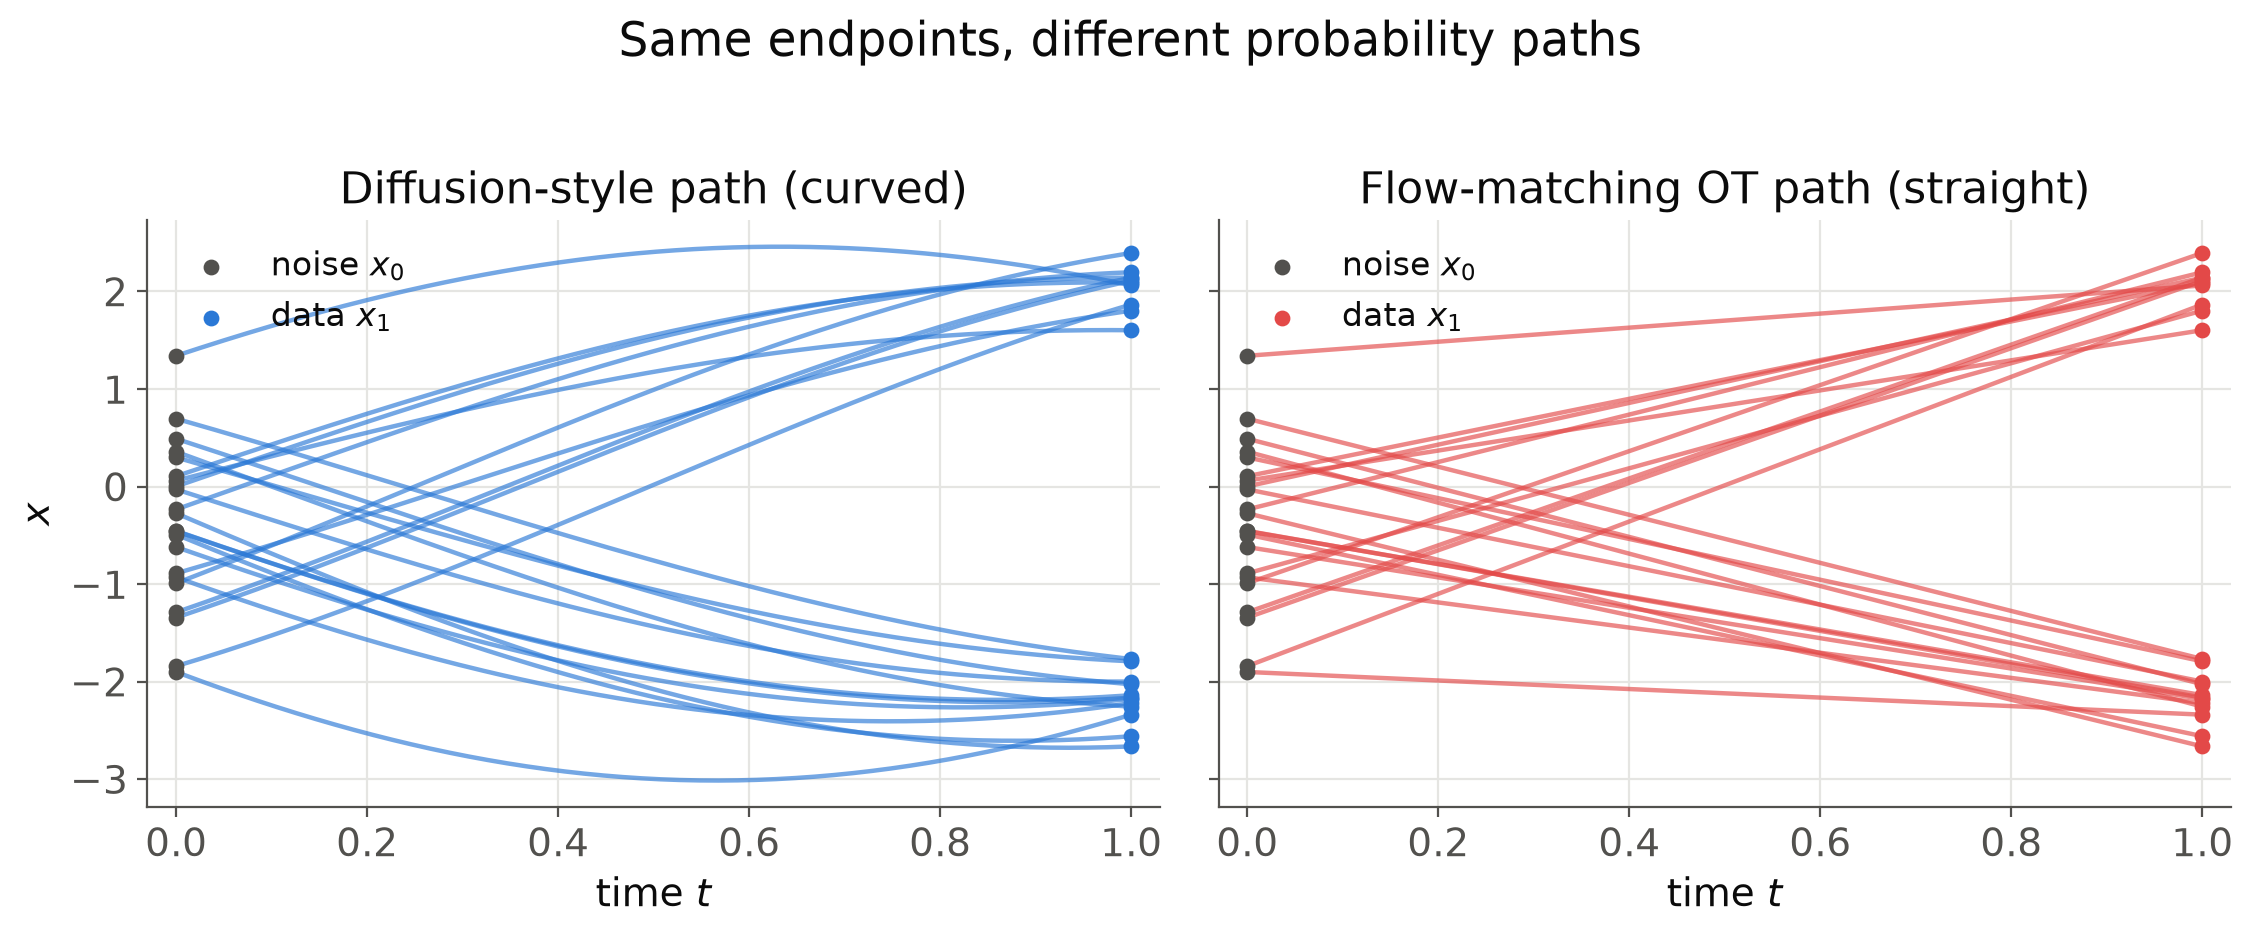
\includegraphics[height=0.55\textheight, width=\textwidth, keepaspectratio]{images/norm-flow/fm_paths_vs_diffusion.png}
\end{figure}
\begin{itemize}
    \item Diffusion-style (variance-preserving) paths take a \textbf{curved detour} between the same endpoints; the optimal-transport / linear paths of flow matching go \textbf{straight}.
    \item Straight paths are easy to integrate: a few Euler steps suffice, which is why flow-matching models sample fast.
\end{itemize}
\end{frame}

\begin{frame}{What the Network Learns}
\begin{figure}
    \centering
    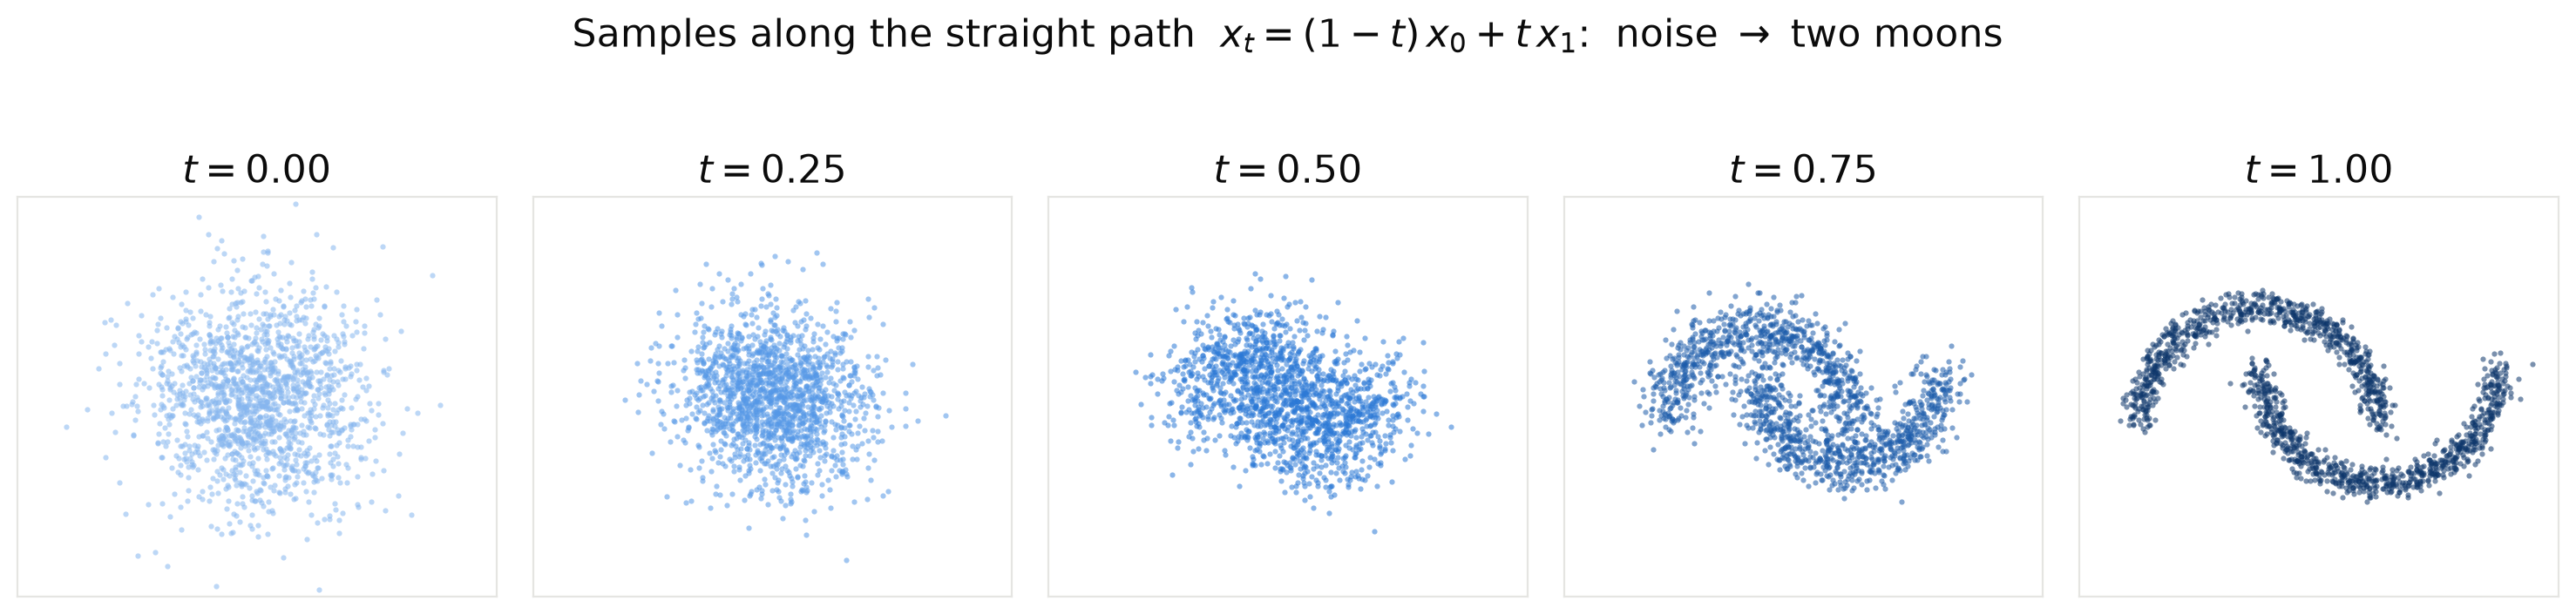
\includegraphics[width=\textwidth, keepaspectratio]{images/norm-flow/fm_interpolation_2d.png}
\end{figure}
\begin{itemize}
    \item Snapshots of the straight path carrying Gaussian noise into a two-moons distribution: the network $v_\theta$ learns the \textbf{velocity field} that produces exactly this motion.
    \item At inference, start from fresh noise and follow the learned field; likelihoods remain available through the instantaneous change of variables from the earlier slide.
\end{itemize}
\end{frame}

\begin{frame}{Flow Matching vs.\ Diffusion and Classical Flows}
\begin{itemize}
    \item \textbf{Classical flows (this lecture):} discrete invertible layers, exact likelihood, but constrained architectures and many layers for expressiveness.
    \item \textbf{CNF with maximum likelihood:} free architecture, but training requires ODE simulation.
    \item \textbf{Diffusion models (covered later):} learn to reverse a gradual noising process; sampling follows a \textbf{curved} path and traditionally needs many steps.
    \item \textbf{Flow matching:} keeps the free architecture, trains by regression (no simulation), and samples with a deterministic ODE along \textbf{straighter} paths.
    \item The families are close relatives: the diffusion (variance-preserving) path is one particular choice of probability path in the flow-matching framework, and score-based training corresponds to a different parameterization of the same object.
\end{itemize}
\end{frame}

\begin{frame}{Why Flow Matching Is the Current State of the Art}
\begin{itemize}
    \item \textbf{Stable Diffusion 3} (Esser et al., 2024): a rectified-flow transformer. Its large-scale ablation found that a rectified-flow path beats established diffusion formulations only once the timestep sampling is biased towards intermediate $t$ (logit-normal sampling); with uniform $t$ it does not.
    \item \textbf{FLUX.1} (Black Forest Labs, 2024): open-weight rectified-flow transformer, among the strongest open text-to-image models at release.
    \item \textbf{Meta Movie Gen} (2024): flow matching as the training objective for large-scale video generation.
    \item \textbf{Voicebox} (Meta, 2023): flow matching for speech generation and editing.
    \item Tooling: Meta's \texttt{flow\_matching} library and the ``Flow Matching Guide and Code'' (Lipman et al., 2024) give a reference implementation of the whole framework.
\end{itemize}
\end{frame}

\begin{frame}{Flow Matching: Takeaways}
\begin{itemize}
    \item Flow matching is the \textbf{continuous-time revival} of everything in this lecture: the same change-of-variables machinery, with the discrete stack replaced by a learned velocity field.
    \item Training reduces to \textbf{regression on interpolations} between noise and data: simple to implement, stable, and free of architectural constraints.
    \item Straight probability paths give \textbf{fast sampling}; likelihoods stay tractable through the instantaneous change of variables.
    \item Normalizing flows did not disappear: reborn as flow matching, they are the objective behind several of today's strongest image, video, and speech generators.
\end{itemize}
\end{frame}
